

\section{Yorug‘lik interferensiyasi}




\begin{enumerate}

\item To‘lqinlar interferensiyasi deb qanday hodisaga aytiladi?
\begin{enumerate}[label=\Alph*)]
\item o‘lchamlari to‘lqin uzunliklari tartibida bo‘lgan to‘siq yoki tirqishga tushgan to‘lqinlarning to‘silgan sohaga og‘ib tarqalish hodisasi.
\item ikki kogerent to‘lqin qo‘shilganda hosil bo‘lgan to‘lqin amplitudasining kuchayishi yoki susayishi hodisasi.
\item to‘siqqa uchragan to‘lqinlarning to‘siqdan bir burchak ostida orqaga qaytib tarqalish hodisasi.
\item ikki to‘lqinning qo‘shilishi natijasida natijaviy tebranishlar amplitudasining keskin ortib yoki kamayib ketish hodisasi.
\item TJY.
\end{enumerate}

\item To‘lqinlar interferensiyasi qachon kuzatiladi?
\begin{enumerate}[label=\Alph*)]
\item chastotalari va fazalar farqi har xil bo‘lgan to‘lqinlar qo‘shilganda.
\item chastotalari bir xil va fazalar farqi o‘zgaruvchan bo‘lgan to‘lqinlar qo‘shilganda.
\item chastotalari har xil va fazalar farqi o‘zgarmas bo‘lgan to‘lqinlar qo‘shilganda.
\item chastotalari va fazalar farqi o‘zgarmas bo‘lgan to‘lqinlar qo‘shilganda.
\item chastotalari bir xil va fazalar farqi o‘zgarmas bo‘lgan to‘lqinlar qo‘shilganda.
\end{enumerate}

\item To‘lqin uzunliklari har xil bo‘lgan to‘lqinlar qanday sharoitda interferensiyalashadi?
\begin{enumerate}[label=\Alph*)]
\item amplitudalari bir xil bo‘lganda.
\item interferensiyalashmaydi.
\item amplituda va boshlang‘ich fazalari bir xil bo‘lganda.
\item har qanday sharoitda.
\item boshlang‘ich fazalari bir xil bo‘lganda.
\end{enumerate}

\item Ushbu interferensiyalanuvchi ikki to‘lqinning fazalar farqi qanday bo‘ladi?

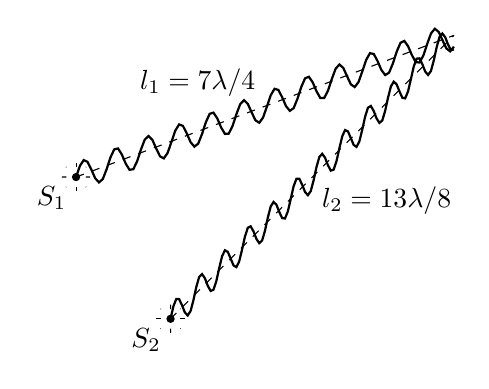
\begin{tikzpicture}[>=latex, scale=0.6]
    % Manbalar
    \node (S1) at (0,3) {}; \node (S2) at (2,0) {};
    \fill (S1) circle (2.5pt) node[below left] {$S_1$};
    \fill (S2) circle (2.5pt) node[below left] {$S_2$};
    % Quyoshcha effekti
    \foreach \a in {0,45,...,315} {
        \draw (S1) -- ++(\a:0.3); \draw (S2) -- ++(\a:0.3);
    }
    % To'lqin yo'llari
    \draw[dashed] (0,3) -- (8,6); \draw[dashed] (2,0) -- (8,6);
    \draw[thick, samples=100, domain=0:8.54] plot ({0 + \x*cos(20.5)}, {3 + \x*sin(20.5) + 0.3*sin(\x*500)});
    \draw[thick, samples=100, domain=0:8.48] plot ({2 + \x*cos(45)}, {0 + \x*sin(45) + 0.3*sin(\x*500)});
    % Yozuvlar
    \node[above left] at (4, 4.5) {$l_1=7\lambda/4$};
    \node[below right] at (5, 3) {$l_2=13\lambda/8$};
\end{tikzpicture}

\begin{enumerate}[label=\Alph*)]
\item $\pi/2$.
\item $\pi/3$.
\item $\pi/4$.
\item $\pi/6$.
\item $\pi$.
\end{enumerate}

\item Ikkita o‘zaro interferensiyalanuvchi monoxromatik yorug‘lik nurlarining yo‘llar farqi $\lambda/6$ ga teng. Tebranishlarning fazalar farqini aniqlang.
\begin{enumerate}[label=\Alph*)]
\item $\pi/6$.
\item $\pi/4$.
\item $\pi/3$.
\item $\pi/2$.
\item $\pi$.
\end{enumerate}

\item Ikkita monoxromatik yorug‘lik to‘lqinlarining bir nuqtadagi yo‘llar farqi $\lambda/4$ ga teng. Tebranishlarning fazalar farqini aniqlang.
\begin{enumerate}[label=\Alph*)]
\item $\pi$.
\item $\pi/2$.
\item $\pi/3$.
\item $\pi/4$.
\item $\pi/6$.
\end{enumerate}

\item Tebranishlar chastotasi 3 Hz bo‘lgan to‘lqin 2,4 m/s tezlik bilan tarqalmoqda. Bir-biridan 20 cm masofada joylashgan nuqtalardagi tebranishlarning fazalar farqi ko‘pi bilan qanday?
\begin{enumerate}[label=\Alph*)]
\item $\pi$.
\item $\pi/2$.
\item $\pi/3$.
\item $\pi/4$.
\item $\pi/6$.
\end{enumerate}

\item Tebranishlarning fazodagi tarqalish tezligi 6 m/s va chastotasi 10 Hz bo‘lsa, bir-biridan 20 cm masofada turuvchi ikki nuqta orasidagi fazalar farqi ko‘pi bilan qanday bo‘ladi?
\begin{enumerate}[label=\Alph*)]
\item $2\pi$.
\item $2\pi/3$.
\item $\pi/6$.
\item $\pi/3$.
\item $4\pi/3$.
\end{enumerate}

\item To‘lqin uzunligi $\lambda$ ga teng bo‘lgan ikkita interferensiyalanuvchi kogerent yorug‘lik to‘lqinlarining fazalar farqi $\pi/4$ ga teng. Optik yo‘llar farqi nimaga teng?
\begin{enumerate}[label=\Alph*)]
\item $\lambda$.
\item $\lambda/2$.
\item $\lambda/4$.
\item $\lambda/8$.
\item $\lambda/16$.
\end{enumerate}

\item Koordinatalar boshida joylashgan tovush manbaidan to‘lqin uzunligi 2 m bo‘lgan tebranishlar tarqalmoqda. Koordinatalari $x_1=2$ m va $x_2=6$ m bo‘lgan nuqtalarning tebranishlar orasidagi fazalar farqi qanday?
\begin{enumerate}[label=\Alph*)]
\item 0.
\item $\pi$.
\item $3\pi$.
\item $4\pi$.
\item $8\pi$.
\end{enumerate}

\item Chastotasi 680 Hz bo‘lgan tovush to‘lqinining ikki nuqtasidan manbagacha bo‘lgan masofalar farqi 25 cm bo‘lsa, bu nuqtalar tebranishlarining fazalar farqi qanday? Tovushning havodagi tezligi 340 m/s.
\begin{enumerate}[label=\Alph*)]
\item $\pi$.
\item $2\pi$.
\item $\pi/3$.
\item $\pi/4$.
\item $\pi/6$.
\end{enumerate}

\item Qanday to‘lqinlar kogerent to‘lqinlar deyiladi?
\begin{enumerate}[label=\Alph*)]
\item bir xil chastotali.
\item bir xil amplitudali.
\item tebranishlari garmonik bo‘lgan.
\item bir xil chastotali va fazalar farqi o‘zgarmas.
\item to‘lqin uzunliklari bir xil.
\end{enumerate}

\item To‘g‘ri tasdiqni ko‘rsating.
\begin{enumerate}[label=\Alph*)]
\item bir xil chastotali va doimiy fazalar farqi hosil qiluvchi yorug‘lik to‘lqinlari o‘zaro kogerent to‘lqinlar deb ataladi.
\item bir xil chastotali yorug‘lik manbalari o‘zaro kogerent manbalar deb ataladi.
\item bir xil uzunlikka ega bo‘lgan va bir tekislik bo‘ylab qutblangan to‘lqinlar kogerent to‘lqinlar deb ataladi.
\item bir xil amplitudali va to‘lqin uzunlikli, o‘zaro tik tekisliklar bo‘ylab qutblangan to‘lqinlar o‘zaro kogerent to‘lqinlar deb ataladi.
\item tabiiy manbadan chiquvchi yorug‘lik to‘lqinlarining o‘zaro kogerentligini ta’minlash mumkin emas.
\end{enumerate}

\item Ikkita kogerent manbadan chiqayotgan amplitudasi $A$ va to‘lqin uzunligi $\lambda=300$ nm bo‘lgan nurlarning interferensiyasi natijasida fazoning ma’lum nuqtasida $\sqrt{3}A$ amplitudaga ega tebranishlar hosil bo‘ldi. Nurlarning minimal yo‘llar farqi (nm) nimaga teng?
\begin{enumerate}[label=\Alph*)]
\item 75.
\item 150.
\item 25.
\item 50.
\item 100.
\end{enumerate}

\item Bir xil $a$ amplitudaga ega bo‘lgan ikkita kogerent to‘lqinlar orasidagi yo‘l farqi yarim to‘lqin uzunligiga teng bo‘lganda, ularning qo‘shilishidan hosil bo‘ladigan natijaviy tebranish amplitudasi qanday bo‘ladi?
\begin{enumerate}[label=\Alph*)]
\item 0.
\item $a/2$.
\item $a$.
\item $2a$.
\item $a^2$.
\end{enumerate}

\item Bir xil $a$ amplitudaga ega bo‘lgan ikkita kogerent to‘lqinlar orasidagi yo‘l farqi juft yarim to‘lqin uzunligiga teng bo‘lganda, ularning qo‘shilishidan hosil bo‘ladigan natijaviy tebranish amplitudasi qanday bo‘ladi?
\begin{enumerate}[label=\Alph*)]
\item 0.
\item $a/2$.
\item $a$.
\item $2a$.
\item $a^2$.
\end{enumerate}

\item O‘zaro kogerent ikki manbadan chiquvchi to‘lqinlar qo‘shilish nuqtasiga bir xil fazada yetib keladilar. Agar to‘lqin amplitudalari $a$ bo‘lsa, natijaviy to‘lqin amplitudasi $A$ qanday bo‘ladi?
\begin{enumerate}[label=\Alph*)]
\item $A=0$.
\item $A=a$.
\item $A=2a$.
\item $0<A<a$.
\item $a<A<2a$.
\end{enumerate}

\item Ikkita kogerent tovush manbai bir xil fazada tebranadi. Birinchi manbadan 3 m va ikkinchi manbadan 4 m masofada joylashgan nuqtada tovush eshitilmaydi. Tovush tezligini 340 m/s deb olsa, tovush chastotasi qanday (Hz)?
$(k=0,1,2...)$
\begin{enumerate}[label=\Alph*)]
\item $(2k+1)340$.
\item $340k$.
\item $680k$.
\item $(2k+1)170$.
\item $340/k$.
\end{enumerate}

\item Elektromagnit tebranishlar generatori $G$ to‘lqin uzunligi 3 cm bo‘lgan monoxromatik to‘lqin tarqatmoqda. $M$ va $N$ nuqtalarda generatordan kelayotgan va $K$ ko‘zgudan qaytgan to‘lqinlar uchrashadi (shaklda masofalar santimetrlarda berilgan). Bu nuqtalarda interferensiya natijalari qanday bo‘ladi? Ko‘zg‘u qaytishida to‘lqin fazasi $\pi$ ga siljiydi deb hisoblang.

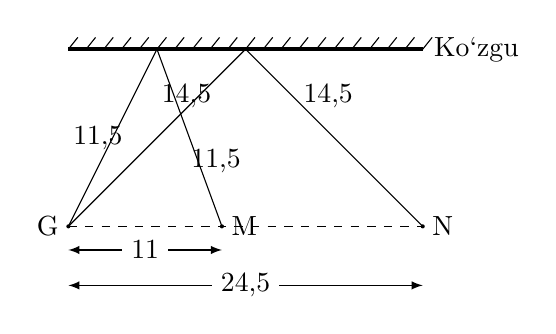
\begin{tikzpicture}[>=latex, scale=0.15]
    % Ko'zgu
    \draw[ultra thick] (0,15) -- (30,15) node[right] {Ko`zgu};
    \foreach \x in {0,1.5,...,30} \draw (\x, 15) -- (\x+0.8, 16);
    % Nuqtalar
    \draw[dashed] (0,0) -- (30,0);
    \fill (0,0) circle (5pt) node[left] {G};
    \fill (13,0) circle (5pt) node[right] {M};
    \fill (30,0) circle (5pt) node[right] {N};
    % Nurlar
    \draw (0,0) -- (7.5,15) -- (13,0);
    \draw (0,0) -- (15,15) -- (30,0);
    % Masofalar
    \node at (2.5, 7.5) {11,5}; \node at (12.5, 5.5) {11,5};
    \node at (10, 11) {14,5}; \node at (22, 11) {14,5};
    \draw[<->] (0,-2) -- (13,-2) node[midway, fill=white] {11};
    \draw[<->] (0,-5) -- (30,-5) node[midway, fill=white] {24,5};
\end{tikzpicture}

\begin{enumerate}[label=\Alph*)]
\item $M$ va $N$ da maksimum.
\item $M$--minimum, $N$--maksimum.
\item $M$--maksimum, $N$--minimum.
\item $M$ va $N$ da minimum.
\item TJY.
\end{enumerate}


\item Ikkita yorug‘lik to‘lqinining ustma-ust tushishi natijasida fazoning ba’zi joylarida intensivlikning kuchayishi, ba’zi joylarida susayishi ... deb ataladi.
\begin{enumerate}[label=\Alph*)]
\item fotoeffekt.
\item yorug‘likning qutblanishi.
\item interferensiya.
\item dispersiya.
\item difraksiya.
\end{enumerate}

\item To‘lqin uzunliklari har xil bo‘lgan ikkita yorug‘lik dastasi qo‘shilishi natijasida interferensiya kuzatiladimi, agar kuzatilsa, qanday shart bajarilgan bo‘ladi?
\begin{enumerate}[label=\Alph*)]
\item interferensiya kuzatilmaydi.
\item boshlang‘ich fazalari bir xil bo‘lishi.
\item tebranish amplitudalari va boshlang‘ich fazalari bir xil bo‘lishi.
\item yo‘llar farqi o‘zgarmas saqlanishi.
\item tebranish amplitudalari bir xil bo‘lishi.
\end{enumerate}

\item Har xil to‘lqin uzunlikdagi ikkita nur dastasi uchun qanday sharoitda interferensiya kuzatilishi mumkin?
\begin{enumerate}[label=\Alph*)]
\item bir xil amplitudali tebranishda.
\item doimiy yo‘llar farqida.
\item bir xil boshlang‘ich fazali tebranishda.
\item bir xil boshlang‘ich faza va amplitudali tebranishda.
\item hech qanday sharoitda.
\end{enumerate}

\item Ikkita kogerent manbadan chiqayotgan yorug‘lik to‘lqinlari berilgan nuqtaga qarama-qarshi fazada keladi. Agar har bir to‘lqinning tebranish amplitudasi $a$ ga teng bo‘lsa, shu nuqtadagi natijaviy tebranish amplitudasi $A$ nimaga teng?
\begin{enumerate}[label=\Alph*)]
\item $A=a$.
\item $0<A<a$.
\item $a<A<2a$.
\item $A=0$.
\item TJY.
\end{enumerate}

\item Ikkita tirqish bilan bog‘liq interferension tajribada tirqishlar orasidagi masofa $d=10\lambda$ ga teng. Tirqishlarga tushayotgan yorug‘likning to‘lqin uzunligi $\lambda$ bo‘lsa, ekrandagi $k$ nuqtada qaysi interferensiya natijasi joylashgan?

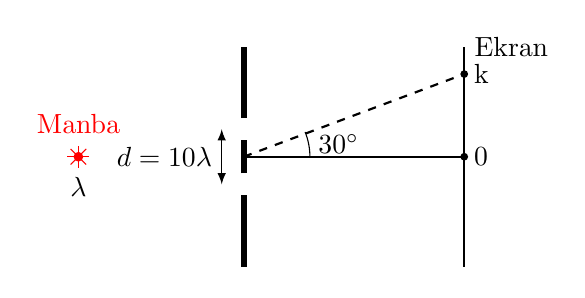
\begin{tikzpicture}[>=latex,scale=0.7]
    % Manba
    \fill[red] (0,0) circle (2.5pt) node[above=5pt] {Manba};
    \foreach \a in {0,45,...,315} \draw[red] (0,0) -- ++(\a:0.2);
    \node[below] at (0,-0.2) {$\lambda$};
    % To'siq (Tirqishlar)
    \draw[line width=2pt] (3,-2) -- (3,-0.7);
    \draw[line width=2pt] (3,-0.3) -- (3,0.3);
    \draw[line width=2pt] (3,0.7) -- (3,2);
    \draw[<->] (2.6, -0.5) -- (2.6, 0.5) node[midway, left] {$d=10\lambda$};
    % Ekran
    \draw[thick] (7,-2) -- (7,2) node[right] {Ekran};
    \draw[thick] (3,0) -- (7,0); \fill (7,0) circle (2pt) node[right] {0};
    \draw[dashed, thick] (3,0) -- (7,1.5); \fill (7,1.5) circle (2pt) node[right] {k};
    % Burchak
    \draw (4.2,0) arc (0:22:1.2) node[midway, right] {$30^\circ$};
\end{tikzpicture}

\begin{enumerate}[label=\Alph*)]
\item 6-maksimum.
\item 8-minimum.
\item 5-maksimum.
\item 7-maksimum.
\item 4-minimum.
\end{enumerate}

\item Ikkita tirqish bilan bog‘liq interferension tajribada tirqishlar orasidagi masofa $d=0{,}1$ mm, tirqishlardan ekrangacha masofa $H=2$ m ga teng. Tirqishlarga tushayotgan yorug‘likning to‘lqin uzunligi $\lambda=6000$ \AA{} bo‘lsa, rasmda ko‘rsatilgan masofa nimaga teng (cm)?

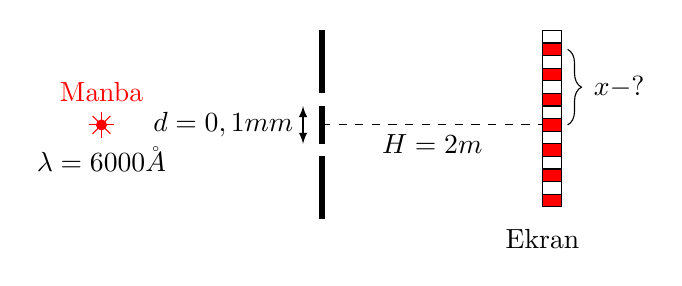
\begin{tikzpicture}[>=latex,scale=0.8]
    % Manba va Tirqishlar
    \fill[red] (0,0) circle (2.5pt) node[above=5pt] {Manba};
    \foreach \a in {0,45,...,315} \draw[red] (0,0) -- ++(\a:0.2);
    \node[below] at (0,-0.2){$\lambda=6000\text{ \AA}$};
    
    \draw[line width=2pt] (3.5,-1.5) -- (3.5,-0.5);
    \draw[line width=2pt] (3.5,-0.3) -- (3.5,0.3);
    \draw[line width=2pt] (3.5,0.5) -- (3.5,1.5);
    \draw[<->] (3.2, -0.3) -- (3.2, 0.3) node[midway, left] {$d=0,1\text{ mm}$};
    % Ekran va Masofa
    \draw[dashed] (3.5,0) -- (7,0) node[midway, below] {$H=2\text{ m}$};
    \node[below] at (7,-1.5) {Ekran};
    % Interferensiya chiziqlari
    \foreach \y in {-1.3, -0.9, ...,1.5} {
        \draw[fill=red] (7,\y) rectangle (7.3, \y+0.2);
        \draw (7, \y+0.2) rectangle (7.3, \y+0.4);
    }
    \draw [decorate, decoration={brace, amplitude=5pt}] (7.4, 1.2) -- (7.4, 0) node [midway, right=6pt] {$x-?$};
\end{tikzpicture}

\begin{enumerate}[label=\Alph*)]
\item 1,2.
\item 1,8.
\item 2,4.
\item 3,6.
\item 4,2.
\end{enumerate}

\item Ikkita tirqish bilan bog‘liq interferension tajribada tirqishlar orasidagi masofa $d=0{,}1$ mm, tirqishlardan ekrangacha masofa $H=2$ m ga teng. Tirqishlarga tushayotgan yorug‘likning to‘lqin uzunligi $\lambda=4000$ \AA{} bo‘lsa, ekrandagi ikkita qo‘shni maksimum orasidagi masofa nimaga teng (m)?

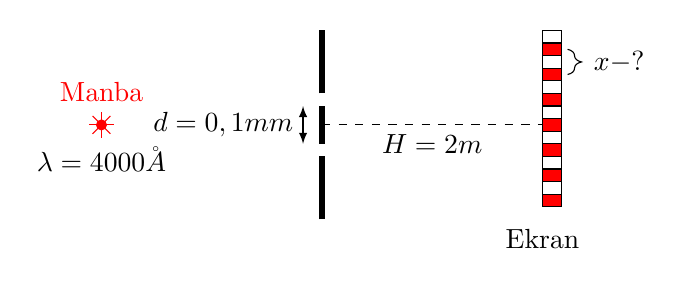
\begin{tikzpicture}[>=latex,scale=0.8]
    % Manba va Tirqishlar
    \fill[red] (0,0) circle (2.5pt) node[above=5pt] {Manba};
    \foreach \a in {0,45,...,315} \draw[red] (0,0) -- ++(\a:0.2);
    \node[below] at (0,-0.2){$\lambda=4000\text{ \AA}$};
    
    \draw[line width=2pt] (3.5,-1.5) -- (3.5,-0.5);
    \draw[line width=2pt] (3.5,-0.3) -- (3.5,0.3);
    \draw[line width=2pt] (3.5,0.5) -- (3.5,1.5);
    \draw[<->] (3.2, -0.3) -- (3.2, 0.3) node[midway, left] {$d=0,1\text{ mm}$};
    % Ekran va Masofa
    \draw[dashed] (3.5,0) -- (7,0) node[midway, below] {$H=2\text{ m}$};
    \node[below] at (7,-1.5) {Ekran};
    % Interferensiya chiziqlari
    \foreach \y in {-1.3, -0.9, ...,1.5} {
        \draw[fill=red] (7,\y) rectangle (7.3, \y+0.2);
        \draw (7, \y+0.2) rectangle (7.3, \y+0.4);
    }
    \draw [decorate, decoration={brace, amplitude=5pt}] (7.4, 1.2) -- (7.4, 0.8) node [midway, right=6pt] {$x-?$};
\end{tikzpicture}

\begin{enumerate}[label=\Alph*)]
\item $4\cdot10^{-6}$.
\item $4\cdot10^{-10}$.
\item $8\cdot10^{-6}$.
\item $8\cdot10^{-10}$.
\item $8\cdot10^{-4}$.
\end{enumerate}

\item Agar yorug‘lik manbalari orasidagi masofani o‘zgartirmay, ular AB ekrandan uzoqlashtirilsa, ekranda hosil bo‘ladigan interferension yo‘llarning kengligi qanday o‘zgaradi?
\begin{enumerate}[label=\Alph*)]
\item avval ortadi, so‘ngra kamayadi.
\item avval kamayadi, so‘ngra ortadi.
\item o‘zgarmaydi.
\item ortadi.
\item kamayadi.
\end{enumerate}

\item O‘lchamlari cheklanmagan ekranda bir-biridan $d$ masofada joylashgan ikkita yorug‘lik manbalari hosil qiluvchi interferensiya manzarasi kuzatiladi. Manbalardan nurlanuvchi monoxromatik yorug‘lik to‘lqin uzunligi $\lambda$. Ekranda kuzatilishi mumkin bo‘lgan natijaviy maksimumlarning sonini aniqlansin.

\begin{tikzpicture}[
    >=Stealth,
    line cap=round,
    font=\small
]

% Manbalar
\coordinate (S1) at (0, 0.72);
\coordinate (S2) at (0,-0.72);

\foreach \P in {S1,S2}{
    \foreach \a in {0,45,...,315}
        \draw[red] ($(\P)+(\a:0.14)$) -- ($(\P)+(\a:0.27)$);
    \fill[red] (\P) circle (0.11);
}

% Manbalar orasidagi masofa
\draw[<->] (0,-0.48) -- node[left=5pt] {$d$} (0,0.48);

% Markaziy yo'nalish
\draw[densely dashed] (0.42,0) -- (4.15,0);

% Ekrandagi qizil-oq interferension palasalar
\foreach \y in {-1.20,-0.80,-0.40,0,0.40,0.80}{
    \fill[red!85] (4.15,\y+0.1) rectangle (4.35,\y+0.3);
    \fill[white]  (4.15,\y+0.3) rectangle (4.35,\y+0.5);
}

% Ekran chegarasi
\draw[thick] (4.15,-1.20) rectangle (4.35,1.20);

% Belgilar
\node[right=4pt] at (4.35,1.13) {$A$};
\node[right=4pt] at (4.35,-1.13) {$B$};
\node[below=5pt] at (4.25,-1.20) {Ekran};

\end{tikzpicture}

\begin{enumerate}[label=\Alph*)]
\item $2\lambda/d$.
\item $d/\lambda$.
\item $\lambda/2d$.
\item $\lambda/d$.
\item $2d/\lambda+1$.
\end{enumerate}

\item Ikkita tirqish bilan bog‘liq interferension tajribada tirqishlar orasidagi masofa $d$ ga, tirqishlardan ekrangacha masofa $l$ ga teng. Tirqishlarga tushayotgan yorug‘likning to‘lqin uzunligi $\lambda$ bo‘lsa, ekranda $L$ uzunlikdagi oraliqda nechta maksimum joylashadi?

\begin{tikzpicture}[
    >=Stealth,
    line cap=round,
    font=\small
]

% Yorug'lik manbai
\coordinate (S) at (0,0);

\foreach \a in {0,45,...,315}
    \draw[red] ($(S)+(\a:0.14)$) -- ($(S)+(\a:0.27)$);
\fill[red] (S) circle (0.11);

\node[above=5pt] at (S) {Manba};
\node[below=6pt] at (S) {$\lambda$};

% Ikki tirqishli to'siq
\fill (1.65, 0.35) rectangle (1.77, 1.13);
\fill (1.65,-0.20) rectangle (1.77, 0.20);
\fill (1.65,-1.13) rectangle (1.77,-0.35);

% Tirqishlar orasidagi d masofa
\draw[<->] (1.48,-0.25) -- node[left=3pt] {$d$} (1.48,0.25);

% Markaziy va chetki nurlar
\coordinate (C) at (1.78,0);
\coordinate (U) at (4.35,1);
\coordinate (D) at (4.35,-1);

\draw[densely dashed] (S) -- (1.47,0);
\draw[densely dashed] (C) -- (4.35,0);
\draw[densely dashed] (C) -- (U);
\draw[densely dashed] (C) -- (D);

% Yuqori va pastki alfa burchaklari
\draw (2.36,0) arc[start angle=0,end angle=20,radius=0.58];
\node at (2.58,0.15) {$\alpha$};

\draw (2.36,0) arc[start angle=0,end angle=-18,radius=0.58];
\node at (2.58,-0.16) {$\alpha$};

% Ekran: qizil-oq interferension palasalar
\foreach \y in {-1.28,-0.96,-0.64,-0.32,0,0.32,0.64}{
    \fill[white] (4.35,\y+0.1) rectangle (4.51,\y+0.26);
    \fill[red]  (4.35,\y+0.26) rectangle (4.51,\y+0.42);
}
\draw[thick] (4.35,-1.1) rectangle (4.51,1.1);

% L oraliqni ko'rsatuvchi qavs
\draw[
    decorate,
    decoration={brace,amplitude=4pt}
] (4.70,0.82) -- (4.70,-0.82)
  node[midway,right=5pt] {$L$};

% Tirqishdan ekrangacha masofa
\node[below=4pt] at (3.00,0) {$l$};

% Ekran yozuvi
\node[below=5pt] at (4.43,-0.96) {Ekran};

\end{tikzpicture}

\begin{enumerate}[label=\Alph*)]
\item $\dfrac{dL}{2l\lambda}$.
\item $\dfrac{dL}{l\lambda}+1$.
\item $\dfrac{d}{\lambda}$.
\item $\dfrac{L\lambda}{d}+1$.
\item $\dfrac{d\lambda}{l}$.
\end{enumerate}

\item Nima uchun bir-biriga bog‘liq bo‘lmagan ikkita yorug‘lik manbaidan (masalan, ikkita yulduzdan) yorug‘lik interferensiyasi kuzatilmaydi?
\begin{enumerate}[label=\Alph*)]
\item bir-biriga bog‘liq bo‘lmagan yorug‘lik manbalari kogerent bo‘lgani uchun.
\item bir-biriga bog‘liq bo‘lmagan yorug‘lik manbalari kogerent bo‘lmagani uchun.
\item yorug‘lik manbalari mustaqil bo‘lgani uchun.
\item ma’lumotlar yetarli emas.
\item TJY.
\end{enumerate}

\item Quyidagi hodisalarning qaysilari interferensiyasi yordamida tushuntiriladi:
\begin{enumerate}
\item[1-] yupqa moy pardasining rangli tovlanishi;
\item[2-] kichik buyum soyasi o‘rtasida yorug‘ dog‘ning hosil bo‘lishi;
\item[3-] Nyuton halqalari;
\item[4-] yorug‘lik nurlarining geometrik soya sohasiga og‘ishi?
\end{enumerate}
\begin{enumerate}[label=\Alph*)]
\item faqat 1.
\item faqat 3.
\item 1 va 3.
\item 1 va 2.
\item hammasi.
\end{enumerate}

\item Ko‘zgu ustida chastotalari $\omega_1$ va $\omega_2$ bo‘lgan monoxromatik to‘lqin tarqatayotgan $S_1$ va $S_2$ yorug‘lik manbalari joylashgan. Nurlarning uchrashuvi natijasida ekrandagi 1, 2 va 3-nuqtalarning qaysilarida interferensiya kuzatilishi mumkin?

\begin{tikzpicture}[font=\small, line cap=round,scale=0.8]

% Asosiy koordinatalar
\coordinate (S1) at (0.4,2.35);
\coordinate (S2) at (0.4,1.20);

\coordinate (P1) at (4.45,2.75);
\coordinate (P2) at (4.45,1.90);
\coordinate (P3) at (4.45,0.80);

\coordinate (M1) at (2.45,0);
\coordinate (M2) at (3.25,0);
\coordinate (M3) at (3.70,0);

% Pastki ko'zgu
\draw[very thick] (0.45,0) -- (4.45,0);
\foreach \x in {0.55,0.70,...,4.35}
    \draw[gray] (\x,0) -- ++(-0.14,-0.11);

% O'ngdagi ekran
\draw[very thick] (4.45,0) -- (4.45,2.85);
\foreach \y in {0.10,0.25,...,2.75}
    \draw[gray] (4.45,\y) -- ++(0.12,0.10);

% Manbalar
\fill (S1) circle (2pt);
\fill (S2) circle (2pt);
\node[left=4pt] at (S1) {$S_1$};
\node[left=4pt] at (S2) {$S_2$};

% Ekrandagi nuqtalar
\node[right=5pt] at (P1) {$1$};
\node[right=5pt] at (P2) {$2$};
\node[right=5pt] at (P3) {$3$};

% To'g'ri keluvchi nurlar
\draw[ray] (S1) -- (P1);
\draw[ray] (S1) -- (P2);
\draw[ray] (S1) -- (P3);

\draw[ray] (S2) -- (P2);
\draw[ray] (S2) -- (P3);

% Ko'zgudan qaytgan nurlar
\draw[ray] (S1) -- (M1);
\draw[ray] (M1) -- (P1);

\draw[ray] (S2) -- (M2);
\draw[ray] (M2) -- (P2);




\end{tikzpicture}

\begin{enumerate}[label=\Alph*)]
\item 1.
\item 2.
\item 3.
\item hammasida.
\item 1 va 3.
\end{enumerate}

\item Bir-biriga nisbatan perpendikular qutblangan, o‘zaro kogerent, bir xil to‘lqin uzunlikda nurlanayotgan ikkita manbadan chiqayotgan qaysi nurlar ekranda interferension manzara hosil qiladi?

\begin{tikzpicture}[font=\small, line cap=round]

% Koordinatalar
\coordinate (S1) at (0.35,2.45);
\coordinate (S2) at (0.35,1.30);

\coordinate (T)  at (4.55,2.45);
\coordinate (C)  at (4.55,1.30);

\coordinate (R1) at (1.5,0);
\coordinate (R2) at (2.8,0);
\coordinate (R3) at (3.45,0);
\coordinate (R4) at (3.85,0);

% Pastki ko'zgu
\draw[very thick] (0.30,0) -- (4.55,0);
\foreach \x in {0.40,0.55,...,4.45}
    \draw[gray] (\x,0) -- ++(-0.14,-0.11);

% Ekran
\draw[very thick] (4.55,0) -- (4.55,2.90);
\foreach \y in {0.10,0.25,...,2.80}
    \draw[gray] (4.55,\y) -- ++(0.12,0.10);

% Ekran yozuvi
\node[right=6pt] at (4.55,2.52) {$e$};
\node[right=6pt] at (4.55,2.10) {$k$};
\node[right=6pt] at (4.55,1.68) {$r$};
\node[right=6pt] at (4.55,1.26) {$a$};
\node[right=6pt] at (4.55,0.84) {$n$};

% Manbalar
\fill (S1) circle (2pt);
\fill (S2) circle (2pt);
\node[left=5pt] at (S1) {$S_1$};
\node[left=5pt] at (S2) {$S_2$};

% Yuqori manbadan chiqayotgan nurlar
\draw[ray] (S1) -- (T);
\node[above] at (2.25,2.45) {$1$};

\draw[ray] (S1) -- (C);
\node[above] at (1.55,2.00) {$2$};

\draw[ray] (S1) -- (R2);
\node[left] at (0.72,1.85) {$3$};
\draw[ray] (R2) -- (T);
\node[below right] at (3.75,0.6) {$4$};

% Pastki manbadan chiqayotgan nurlar
\draw[ray] (S2) -- (C);
\node[above] at (2.25,1.30) {$5$};

\draw[ray] (S2) -- (T);
\node[above] at (2.88,2.02) {$6$};

\draw[ray] (S1) -- (R3);
\node[below left] at (1.5,0.92) {$7$};
\draw[ray] (R3) -- (C);

\draw[ray] (R2) -- (C);
\draw[ray] (S2)--(R2);
\draw[ray] (S2) -- (R1);
\node[left] at (0.8,0.68) {$8$};
\draw[ray] (R1) -- (T);

\end{tikzpicture}

\begin{enumerate}[label=\Alph*)]
\item 1-3, 2-4, 5-7, 6-8.
\item 1-3, 5-7.
\item 3-4, 2-6.
\item 1-4, 2-5.
\item 1-4-3, 2-5-6.
\end{enumerate}

\item Quyidagi hodisalarning qaysilari interferensiya hodisasi asosida tushuntiriladi?
\begin{enumerate}
\item sovun pufagi yoki yog‘ pardasidagi kamalak ranglarning kuzatilishi;
\item Nyuton halqalari;
\item kichik doiraviy diskdan hosil bo‘lgan soyaning markazida yorug‘ dog‘ hosil bo‘lishi;
\item yorug‘lik nurlarining to‘siq chegarasida geometrik soya sohasiga og‘ishi.
\end{enumerate}
\begin{enumerate}[label=\Alph*)]
\item 1, 2.
\item 1.
\item 1, 2, 3.
\item 3, 4.
\item 4.
\end{enumerate}

\item Nyuton halqalarini kuzatish qurilmasi monoxromatik yorug‘lik bilan yoritiladi. Agar yorug‘lik nurining to‘lqin uzunligi 600 nm, linza egrilik radiusi 1,5 m bo‘lsa, rasmda ko‘rsatilgan halqaning radiusi qanday (mm)?

\begin{tikzpicture}[>=Stealth, line cap=round, font=\small]

% Markaz
\coordinate (O) at (0,0);

% Nyuton halqalari
\fill[gray!55] (O) circle (0.42);

\fill[gray!55, even odd rule]
    (O) circle (1.22)
    (O) circle (0.78);

\fill[gray!55, even odd rule]
    (O) circle (1.78)
    (O) circle (1.58);

\fill[gray!55, even odd rule]
    (O) circle (2.05)
    (O) circle (1.92);

% Tashqi kontur
\draw[gray, thick] (O) circle (2.05);

% Markaz nuqtasi
\fill (O) circle (2pt);

% Radius ko'rsatkichi
\draw[->, thick] (O) -- (35:1.80)
    node[pos=0.55, above left] {$r$};

\end{tikzpicture}

\begin{enumerate}[label=\Alph*)]
\item 1,5.
\item 3.
\item 3,2.
\item 4,6.
\item 0,9.
\end{enumerate}

\item Nyuton halqalarini kuzatish qurilmasi monoxromatik yorug‘lik bilan yoritiladi. Agar yorug‘lik nurining to‘lqin uzunligi 500 nm, linza egrilik radiusi 4 m bo‘lsa, sakkizinchi qora halqaning radiusi qanday (mm)?
\begin{enumerate}[label=\Alph*)]
\item 4.
\item 3.
\item 2.
\item 5.
\item 6.
\end{enumerate}

\item Nyuton halqalarini kuzatish qurilmasi monoxromatik yorug‘lik bilan yoritiladi. Bunda ikkita qo‘shni qora halqalarning radiuslari mos ravishda 1,732 mm va 2 mm. Bular nechanchi qora halqalar?
\begin{enumerate}[label=\Alph*)]
\item 1 va 2.
\item 2 va 3.
\item 3 va 4.
\item 4 va 5.
\item 5 va 6.
\end{enumerate}

\item To‘lqin uzunligi $\lambda=600$ nm bo‘lgan yorug‘lik yupqa pardaga rasmdagikabi tushmoqda. Pardadan qaytgan yorug‘lik ko‘zga yorqin ranglarda ko‘rindi. Pardaning qalinligi quyidagilardan qaysi biri bo‘lishi mumkin? Pardaning sindirish ko‘rsatkichi $n=1{,}5$ ga teng.

\begin{tikzpicture}[
    >=Stealth,
    line cap=round,
    font=\small
]

% Ko'z belgisi
\draw[thick] (2.10,2.60) .. controls (2.28,2.86) and (2.52,2.86) .. (2.70,2.60)
             .. controls (2.52,2.36) and (2.28,2.36) .. (2.10,2.60);
\draw[thick] (2.42,2.42) arc[start angle=-70,end angle=70,radius=0.20];
\fill (2.40,2.60) circle (0.045);
\draw[thick] (2.68,2.88) .. controls (2.82,2.62) and (2.83,2.42) .. (2.72,2.25);

% Tushuvchi yorug'lik nurlari
\foreach \x in {1.65,1.90,2.15,2.40,2.65,2.90,3.15}{
    \draw[->] (\x,2.05) -- (\x,1.42);
}
\node[right] at (3.22,1.73) {$\lambda=600\ \mathrm{nm}$};

% Yupqa parda
\fill[gray!48]
    (0.20,1.18)
    decorate[decoration={snake,amplitude=1.5pt,segment length=7pt}]
        {-- (0.20,0.18)}
    -- (4.75,0.18)
    decorate[decoration={snake,amplitude=1.5pt,segment length=7pt}]
        {-- (4.75,1.18)}
    -- cycle;

\draw[gray!70]
    (0.20,1.18)
    decorate[decoration={snake,amplitude=1.5pt,segment length=7pt}]
        {-- (0.20,0.18)};
\draw[gray!70]
    (4.75,0.18)
    decorate[decoration={snake,amplitude=1.5pt,segment length=7pt}]
        {-- (4.75,1.18)};

% Muhit yozuvlari
\node at (0.58,1.34) {havo};
\node at (0.58,0.03) {havo};
\node at (3.85,0.68) {$n=1{,}5$};

% Qalinlik d
\draw[<->,thick] (0.63,1.12) -- node[right=4pt] {$d$} (0.63,0.24);



\end{tikzpicture}

\begin{enumerate}[label=\Alph*)]
\item 800 nm.
\item 700 nm.
\item 400 nm.
\item 600 nm.
\item 200 nm.
\end{enumerate}

\item To‘lqin uzunligi $\lambda=640$ nm bo‘lgan yorug‘lik yupqa pardaga normal holda tushmoqda. Parda tepasidan qaralganda ko‘zga parda sirti qorong‘i ko‘rindi. Pardaning qalinligi quyidagilardan qaysi biri bo‘lishi mumkin? Pardaning sindirish ko‘rsatkichi $n=1{,}6$ ga teng.

\begin{tikzpicture}[
    >=Stealth,
    line cap=round,
    font=\small
]

% Ko'z belgisi
\draw[thick] (2.10,2.60) .. controls (2.28,2.86) and (2.52,2.86) .. (2.70,2.60)
             .. controls (2.52,2.36) and (2.28,2.36) .. (2.10,2.60);
\draw[thick] (2.42,2.42) arc[start angle=-70,end angle=70,radius=0.20];
\fill (2.40,2.60) circle (0.045);
\draw[thick] (2.68,2.88) .. controls (2.82,2.62) and (2.83,2.42) .. (2.72,2.25);

% Tushuvchi yorug'lik nurlari
\foreach \x in {1.65,1.90,2.15,2.40,2.65,2.90,3.15}{
    \draw[->] (\x,2.05) -- (\x,1.42);
}
\node[right] at (3.22,1.73) {$\lambda=640\ \mathrm{nm}$};

% Yupqa parda
\fill[gray!48]
    (0.20,1.18)
    decorate[decoration={snake,amplitude=1.5pt,segment length=7pt}]
        {-- (0.20,0.18)}
    -- (4.75,0.18)
    decorate[decoration={snake,amplitude=1.5pt,segment length=7pt}]
        {-- (4.75,1.18)}
    -- cycle;

\draw[gray!70]
    (0.20,1.18)
    decorate[decoration={snake,amplitude=1.5pt,segment length=7pt}]
        {-- (0.20,0.18)};
\draw[gray!70]
    (4.75,0.18)
    decorate[decoration={snake,amplitude=1.5pt,segment length=7pt}]
        {-- (4.75,1.18)};

% Muhit yozuvlari
\node at (0.58,1.34) {havo};
\node at (0.58,0.03) {havo};
\node at (3.85,0.68) {$n=1{,}6$};

% Qalinlik d
\draw[<->,thick] (0.63,1.12) -- node[right=4pt] {$d$} (0.63,0.24);

\end{tikzpicture}

\begin{enumerate}[label=\Alph*)]
\item 500 nm.
\item 700 nm.
\item 800 nm.
\item 100 nm.
\item 300 nm.
\end{enumerate}

\item To‘lqin uzunligi $\lambda=520$ nm bo‘lgan yorug‘lik yupqa pardaga rasmdagikabi tushmoqda. Pardadan qaytgan yorug‘lik ko‘zga yorqin ranglarda ko‘rinishi uchun pardaning qalinligi $d=100$ nm bo‘lishi kerak. Bunda pardaning sindirish ko‘rsatkichi nima bo‘lgan?

\begin{tikzpicture}[
    >=Stealth,
    line cap=round,
    font=\small
]

% Ko'z belgisi
\draw[thick] (2.10,2.60) .. controls (2.28,2.86) and (2.52,2.86) .. (2.70,2.60)
             .. controls (2.52,2.36) and (2.28,2.36) .. (2.10,2.60);
\draw[thick] (2.42,2.42) arc[start angle=-70,end angle=70,radius=0.20];
\fill (2.40,2.60) circle (0.045);
\draw[thick] (2.68,2.88) .. controls (2.82,2.62) and (2.83,2.42) .. (2.72,2.25);

% Tushuvchi yorug'lik nurlari
\foreach \x in {1.65,1.90,2.15,2.40,2.65,2.90,3.15}{
    \draw[->] (\x,2.05) -- (\x,1.42);
}
\node[right] at (3.22,1.73) {$\lambda$};

% Yupqa parda
\fill[gray!48]
    (0.20,1.18)
    decorate[decoration={snake,amplitude=1.5pt,segment length=7pt}]
        {-- (0.20,0.18)}
    -- (4.75,0.18)
    decorate[decoration={snake,amplitude=1.5pt,segment length=7pt}]
        {-- (4.75,1.18)}
    -- cycle;

\draw[gray!70]
    (0.20,1.18)
    decorate[decoration={snake,amplitude=1.5pt,segment length=7pt}]
        {-- (0.20,0.18)};
\draw[gray!70]
    (4.75,0.18)
    decorate[decoration={snake,amplitude=1.5pt,segment length=7pt}]
        {-- (4.75,1.18)};

% Muhit yozuvlari
\node at (0.58,1.34) {havo};
\node at (0.58,0.03) {havo};
\node at (3.85,0.68) {$n$};

% Qalinlik d
\draw[<->,thick] (0.63,1.12) -- node[right=4pt] {$d$} (0.63,0.24);


\end{tikzpicture}

\begin{enumerate}[label=\Alph*)]
\item $n=1{,}2$.
\item $n=1{,}3$.
\item $n=1{,}5$.
\item $n=1{,}8$.
\item $n=2$.
\end{enumerate}

\item Moddaning sindirish ko‘rsatkichi $n=1{,}5$ bo‘lgan $d=210$ nm qalinlikdagi yupqa parda sirtiga tik yo‘nalgan oq nur dastasi bilan yoritilsa, qaytuvchi nurlarda parda qanday ko‘rinadi?
\begin{enumerate}[label=\Alph*)]
\item binafsha.
\item ko‘k.
\item yashil.
\item sariq.
\item qizil.
\end{enumerate}

\end{enumerate}




\textbf{Kalitlar}

\begin{center}
\begin{tabular}{|c|c|c|c|c|c|c|c|c|c|}
\hline
1b & 2e & 3b & 4c & 5c & 6b & 7b & 8b & 9d & 10d \\
\hline
11a & 12d & 13a & 14d & 15a & 16d & 17c & 18d & 19b & 20c \\
\hline
21a & 22e & 23d & 24c & 25d & 26c & 27d & 28e & 29b & 30b \\
\hline
31c & 32e & 33a & 34a & 35a & 36a & 37c & 38b & 39c & 40b \\
\hline
41a & & & & & & & & & \\
\hline
\end{tabular}
\end{center}



